% Introduction v2, installed 2026-09-08. Version history: paper/introduction_versions/
% Built to the budget in .workspace/notes/intro_writing_map.md: 6 paragraphs, ~700 words.
% Method: Liam's existing sentences trimmed and resequenced, not replaced. New prose is
% confined to the results paragraph, where the numbers changed.
%
% CITATIONS: 13, unchanged from the current draft. The map calls for 18. The five
% additions are NOT made here because no citation should be attached to a claim without
% the source having been read for that claim. Candidate insertion points are marked
% [CITE-GAP] below with the claim each would support. See the standing TODO,
% "Verify that each cited work supports the claim the paper attaches to it."

\section{Introduction}

% P1 FIELD. 112w, 4 cites. Opener kept: see paper/reference/emami_writing_patterns.md,
% four analogues in 24 of his introductions. Cut the closing self-location sentence
% ("is the concern of human-AI interaction, and it is where we situate this work"),
% which is a relevance tag rather than a claim.
% [CITE-GAP] a group of 2-3 benchmark papers alongside liang2023holistic on the claim
% that single-turn scoring against a reference is the standard evaluation form.
Large language models are evaluated, for the most part, alone. A model is handed a fully
specified task, produces one answer, and is scored against a reference. On benchmarks of
this form current models perform well \cite{liang2023holistic}. The tasks
that motivate their deployment are rarely solved in a single exchange. Increasingly they
are workplace tasks carried out with a user who supplies the goal, reacts to the output,
and asks for changes \cite{anthropic2025economicindex, laban2025lost}. The quality such a
user receives is a property of the exchange, not of the model alone, and it turns on what
the user contributes. What users contribute is often thin: real prompts are
frequently underspecified, and underspecification degrades the outputs that follow
\cite{yang2025underspecification}.

% P2 PROBLEM, ending on the figure. 135w, 3 cites. The eight-word float-anchor paragraph
% is absorbed here, which takes the introduction from 7 paragraphs to 6, the corpus
% median. Theatrical closer cut ("and it is where the collaboration quietly fails").
The user-side contribution that matters most is the ability to say what is wrong with an
output. A user who can name a specific weakness can direct the model to fix it. A user who
cannot has one move available, and scalable-oversight research identifies that condition
as central: users often cannot articulate precise intent or reliably validate a complex
output \cite{zhou2026oversight}. They ask the model to improve the work without saying
what improving it would mean. This undirected request, some version of \emph{make it
better}, is what vendor guidance is written against. Both providers advise stating what
you want rather than letting the model infer it
\cite{openai2025prompting, anthropic2025prompting}.
Figure~\ref{fig:teaser} follows one such request through four revisions, over which the
explanations the prompt asked for disappear and the judged quality falls below sufficient.

\begin{figure*}[!t]
    \centering
    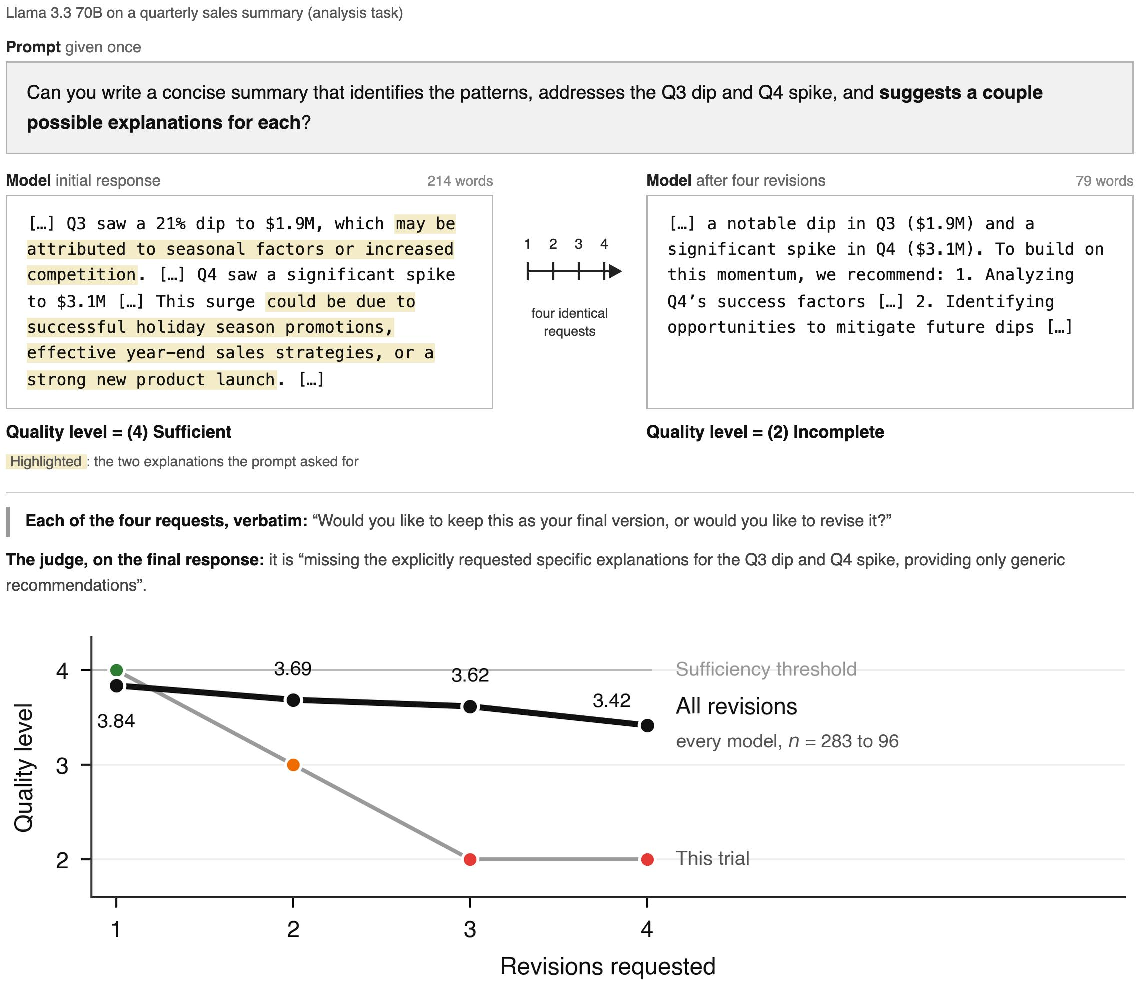
\includegraphics[width=\textwidth]{figures/fig1.pdf}
    \caption{\textbf{Undirected revision removes content the user asked for.} One trial of the
    quarterly sales summary task (Llama~3.3~70B, run~3). The prompt is shown in excerpt;
    model output is monospace, shown after meta-commentary stripping to match the scores.
    The numbered arrow marks the four identical requests separating the two responses; the
    three intermediate responses are not shown. Bracketed ellipses mark omissions, and the
    bold in the prompt and the highlighting are added. Nothing else is altered. The lower
    panel plots revisions only, since the initial response is not a revision. The solid
    black series is the mean over every genuine revision at that index across all six
    models, whose $n$ falls from 283 to 96 as models stop producing genuine revisions; the
    lighter series is this trial, its markers coloured by judged level. The full exchange
    and every judge rationale appear in Appendix~\ref{sec:appendix-teaser}.}
    \label{fig:teaser}
\end{figure*}

% P3 PRIOR WORK. 123w, 4 cites. Dialectic preserved; rules/03 Part 1 rates this paragraph
% at corpus standard. Trimmed only.
% [CITE-GAP] the two or three multi-turn works the gap paragraph characterizes but does
% not cite, attached to the Laban sentence.
Whether models can improve their own outputs has been studied as self-refinement.
\citet{madaan2024self} show that a model given the chance to critique and rewrite its work
can raise its quality, and locate the benefit in feedback that is \emph{actionable} and
\emph{specific}, naming a concrete change to a concrete part of the output. Subsequent work
finds the benefit fragile. \citet{huang2024large} report that without external feedback
models struggle to correct their own reasoning and at times degrade it, and that apparent
gains often trace to information leaked through oracle labels. A critical survey by
\citet{kamoi2024selfcorrection} reaches a compatible conclusion across tasks, locating the
bottleneck in feedback generation rather than in the capacity to revise. In parallel,
\citet{laban2025lost} show that models lose accuracy across multi-turn conversations when
requirements arrive piecewise.

% P4 GAP. 92w, 2 cites. Fence-then-consequence construction kept; rules/03 Part 1 rates it
% one of the better gap paragraphs in the corpus.
These results bracket the question we ask without answering it. Revision driven only by the
model's own judgment, with no signal supplied from outside, is what
\citet{kamoi2024selfcorrection} and \citet{huang2024large} term \emph{intrinsic}
self-correction, and the literature studies it alongside revision that does carry a signal.
Neither that work nor the multi-turn literature measures the case a non-expert user
actually creates: a fully specified task whose output is already adequate, followed by
repeated requests to revise that carry no feedback at all. Measuring it requires
controlling for an artifact the revision act introduces into automated evaluation.

% P5 APPROACH. 103w, 0 cites. Three RQs compressed from three sentences to one.
We study this case directly. A model completes one of forty fully specified tasks and is
then offered, at each of four subsequent turns, a neutral choice to keep its output or
revise it, with no indication of what to change. The design spans six models, 720
conversations and 3,600 responses. We ask whether such a model revises at all (RQ1),
whether the output improves or degrades when it does (RQ2), and whether failure traces to
capacity or to the absence of direction (RQ3).
We strip the meta-commentary models attach to revisions, and validate every quality
judgment against human raters.

% P6 RESULTS. 155w, 0 cites. Rewritten: carries the four numbers the final abstract leads
% on, each with its referent. The practical recommendation ("withhold the request to revise
% until there is a specific weakness to direct it at") is CUT and belongs in the Discussion.
% The judge-bias finding is kept as a clause without figures.
Most of the work being revised did not need revising: 88\% of the 720 first drafts are
already sufficient. Asked to improve them without direction, models mostly do not revise
at all, restating the work or declining while presenting it as compliance. When they do
revise, 70\% of the changes that move quality move it down, and where the work was already
sufficient, 27\% of revisions leave it below the threshold. For all six models the first
draft is the quality-maximizing stopping point. Blind readers prefer it to the last in
56\% of decisions, an interval that includes chance. We read this as a failure of
direction rather than capacity, because a single specific critique reverses the decline.
Intrinsic self-correction, on its own, is not enough. It requires extrinsic direction.
